\documentclass[a4paper,11pt]{report}
\usepackage[T1]{fontenc}
\usepackage[utf8]{inputenc}
\usepackage{lmodern}
\usepackage[francais]{babel}
\usepackage{graphicx}
\usepackage{array}

\title{Data wars }

\author{Guillaume LAROYENNE, Nathan PRETOT \\ Jeremy RENAUD, Tom SALVI, Pierre VALENZA}

\begin{document}

\maketitle
\tableofcontents
\begin{abstract}

\end{abstract}



\chapter{La base de donnée}
    Dans cette partie nous allons détailler la base de données utilisée par \textit{Data wars}. Nous allons diviser le MCD (\textit{Figure~\ref{fig1}}) en plusieurs sous-parties que nous allons détailler par la suite. Nous allons donc procéder à la découpe suivante : 
    
    \begin{figure}[th]
      \begin{center}
        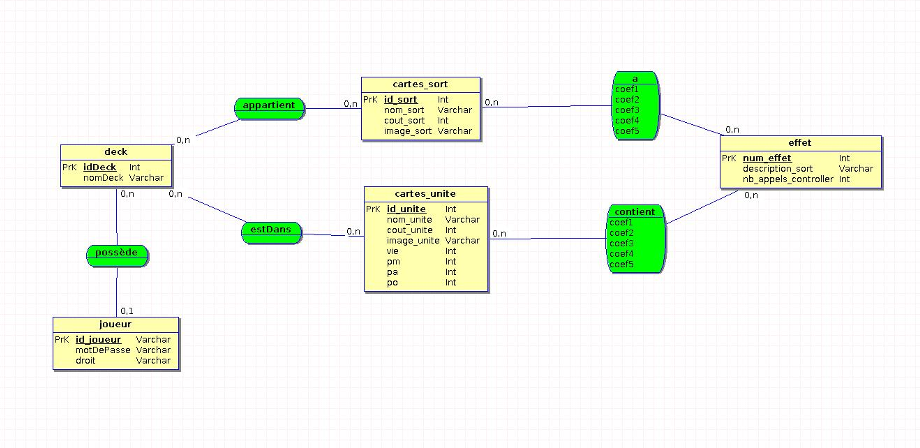
\includegraphics[scale=0.4]{Assets/MCD.png}
        \caption{MCD du jeu \textit{data wars}}
        \label{fig1}
      \end{center}
    \end{figure}
    
    \begin{itemize}
      \item Joueur et Deck
      \item Cartes
      \item Effets
    \end{itemize}

    \section{Joueur et deck}
      La base de données va stocker le nom des joueurs et leurs mots de passe ainsi que les droits pour les accès au site web. Un deck sera relié à chaque joueur.
    
    \begin{figure}[th]
      \begin{center}
        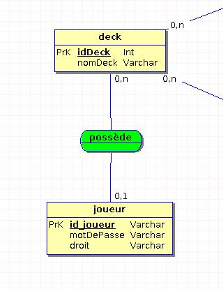
\includegraphics[scale=0.6]{Assets/MCD_Joueur.png}
        \caption{Zoom sur le joueur et le deck}
        \label{fig2}
      \end{center}
    \end{figure}
    
    
    \section{Les cartes}
      Il existe deux types de cartes, les cartes sorts et les cartes unités. Les cartes sorts contiennent moins d'informations que leurs homologues. Elles ne contiennent que le coût, le chemin vers l'image et le nom en plus de leurs identifiants. Les cartes unités, elles, contiennent les caractéristiques nécessaires à la création des unités. Elles sont liées au deck, chacune via une association. Puis d'un autre coté, elles sont aussi reliées aux effets.
      
    \begin{figure}[th]
      \begin{center}
        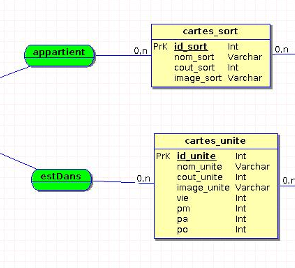
\includegraphics[scale=0.6]{Assets/MCD_Cartes.png}
        \caption{Zoom sur les cartes}
        \label{fig3}
      \end{center}
    \end{figure}
      
      \section{Les effets}
        Les effets sont les derniers éléments de cette base de données. Chaque élément \textit{<<effet>>} inséré dans la base de données correspond à un type d'effet, par exemple : <<soigne de X points de vies>> ou <<inflige X points de dégâts>>. C'est lorsque ce type \textit{<<effet>>} sera lié à une carte via les associations \textit{<<a>>} et \textit{<<contient>>} que les valeurs remplaceront les <<X>> via les coefficients. Les coefficients utilisés (c'est-à-dire dans nos deux exemples, seulement le premier coefficient) devront être remplis et les autres seront mis à -1. La variable \textit{nb\_appels\_controller} sert elle, à indiquer le nombre de clics nécessaires pour jouer une carte qui contient cet effet.

    \begin{figure}[th]
      \begin{center}
        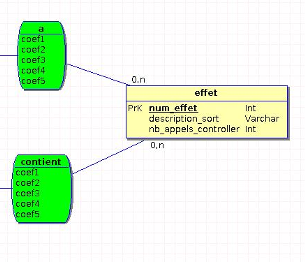
\includegraphics[scale=0.6]{Assets/MCD_Effet.png}
        \caption{Zoom sur les effets}
        \label{fig4}
      \end{center}
    \end{figure}

\chapter{Le modèle}
    Le modèle est composé d'un ensemble de classes toutes reliées de près, ou de loin, à la classe dite <<mère>> du modèle la classe \textit{Game}. Nous pouvons ensuite décomposer le schéma UML (\textit{Figure ~\ref{fig5}}) en trois gros blocs :
    \begin{itemize}
      \item Le bloc concernant la grille (la carte)
      \item Le bloc concernant les joueurs
      \item Le bloc concernant le serveur 
    \end{itemize}
    Le troisième bloc sera détaillé en aval. Nous allons ici nous concentrer sur la partie jeu du programme, soit les deux premières parties.
    
    \begin{figure}[th]
      \begin{center}
        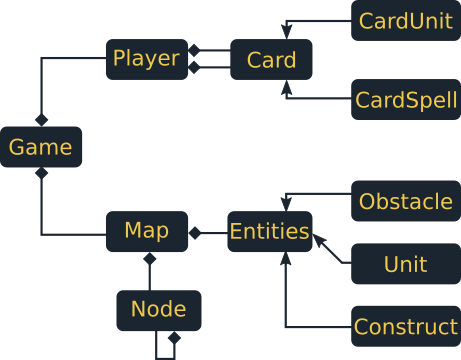
\includegraphics[scale=0.4]{Assets/UML.png}
        \caption{Le schémas UML du jeu}
        \label{fig5}
      \end{center}
    \end{figure}
    
    \section{Le bloc grille}
        La carte du jeu, que nous appellerons ici <<grille>> ou encore \textit{<<map>>} et l'élement essentiel du bloc grille. Cette objet Java contient un tableau à deux dimensions qui représente la grille ainsi que d'autre attributs qui seront expliqués plus en détails par la suite. Cette classe contient la plupart des fonctions de traitement des entités, qui sont les éléments qui composent la grille. Rentrons plus en détails dans ce bloc.
    \begin{figure}[th]
      \begin{center}
        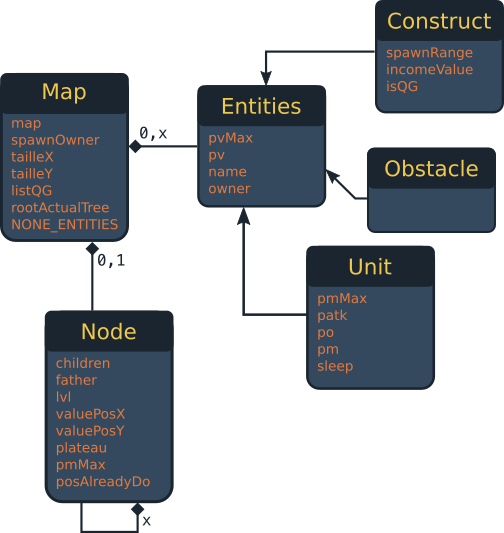
\includegraphics[scale=0.4]{Assets/umlBlocGrille.png}
        \caption{Zoom sur le bloc grille}
        \label{fig6}
      \end{center}
    \end{figure}
        \subsection{Les entités}
          \begin{center}
           \textit{Classe : Entities, Unit, Construct, Obstacle}
          \end{center}
          Les entités sont les éléments contenus par la grille. Elle sont de type \textit{entities}, c'est-à-dire qu'elles appartiennent à cette classe. Cette classe contient les propriétés suivantes :
          \begin{itemize}
            \item <<points de vie actuels>>
            \item <<points de vie>>
            \item <<nom>>
            \item <<propriétaire>>
          \end{itemize}
          Il faut savoir que toutes les propriétés <<points de vie>> sont dédoublées. En effet, il faut garder pour la propriété <<points de vie>> la valeur de départ pour ne pas dépasser cette limite si nous soignons l'unité.
          La classe \textit{Entities} va avoir trois subdivisions, que l'on appele <<type d'entité>> :
          \begin{description}
            \item[Les unités :] modélisées par la classe \textit{Unit}, elle correspond aux unités que le joueur peut poser. Elles ont des attributs supplémentaires, les <<points de mouvement>> et <<points de mouvement maximum>>, ainsi que des points d'attaque. Elles peuvent attaquer les autres unités qui perdront des points de vie et pourront potentiellement contre-attaquer.
            \item[Les obstacles :] modélisés par la classe \textit{Obstacle}, correspond aux obstacles qui sont là pour bloquer les unités.
            \item[Les bâtiments :] modélisés par la classe \textit{Construct}, elle correspond aux QG et aux bâtiments de ressources. Ils ont plusieurs attributs supplémentaires tels que le \textit{spawnrange} qui détermine la zone où nous pouvons placer des unités quand le bâtiment nous appartient, l'\textit{incomeValue} qui est le nombre de ressources données par ce bâtiment par tour. Enfin la variable \textit{isQg} détermine si ce bâtiment est un QG ou non.
          \end{description}
        \subsection{L'accès aux unités}
          \begin{center}
           \textit{Classe : Map}
          \end{center}
          Pour accéder aux unités, il faut passer par l'attribut \textit{map} de la classe \textit{Map}. Pour ce repèrer, il faut comprendre le système algorithmique de gestion des coordonnées (\textit{Figure~\ref{xyExample}}). Or, lors de l'appel à certaines méthodes, l'utilisateur doit envoyer un tableau de coordonnées sous la forme [x,y]. Il faut donc faire attention à ne pas mélanger les deux.
        
        \begin{figure}[th]
          \begin{center}
            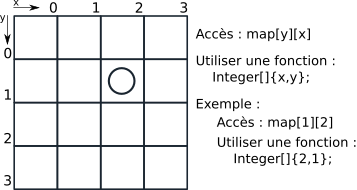
\includegraphics[scale=0.6]{Assets/xyExemple.png}
            \caption{Exemple d'accès aux unités}
            \label{xyExample}
          \end{center}
        \end{figure}
        
        
        \subsection{Les déplacements}
        \begin{center}
          \textit{Classe : Map - Fonction : setUnitTreeOfMove(), move()}
        \end{center}
          La gestion du plus court chemin et des obstacles a nécessité la création d'un système d'arbre afin de calculer les différentes possibilités de déplacements et de choisir le chemin le plus optimisé. Pour créer cet arbre, nous avons créé une classe \textit{Node} qui va gérer ce traitement. En fonction d'une coordonnée passée en paramètre, ainsi que d'un nombre de points de mouvement, elle peut calculer l'arbre des possibilités (\textit{Figure~\ref{treeExample}}), où chaque nœud correspond à une position. De plus, elle va nous générer une liste contenant toutes les positions accessibles par l'unité afin de pouvoir l'afficher. Ensuite cet arbre subira un parcours en largeur afin de déterminer le plus court chemin (\textit{Figure~\ref{parcourExample}}) pour aller à une position, en récupèrent de nombre de points de mouvements nécessaire. Le déplacement permet également, si l'unité attaque au corps à corps et si la position de destination est occupée par une autre entité, de l'attaquer.
          
          \begin{figure}[th]
          \begin{center}
            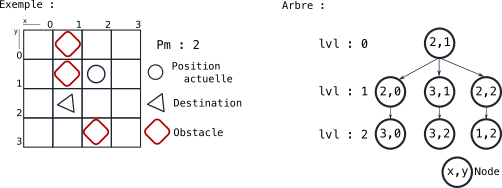
\includegraphics[scale=0.6]{Assets/treeExample.png}
            \caption{Exemple d'une création d'arbre via la classe \textit{Node}}
            \label{treeExample}
          \end{center}
        \end{figure}
            
        \begin{figure}[th]
          \begin{center}
            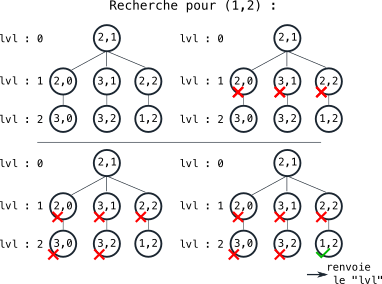
\includegraphics[scale=0.6]{Assets/parcourTree.png}
            \caption{Exemple d'un traitement de l'arbre}
            \label{parcourExample}
          \end{center}
        \end{figure}
        

      
        \subsection{Utilisation des nodes}
        \begin{center}
          \textit{Classe : Node - Fonction : calcNextLevel(), searchLowCostPath(), searcheLowCostPathForAttack(), setUpTreeOfMovement()}
        \end{center}
          L'utilisation de la classe \textit{Node} nécessite une certaine rigueur de part sa construction. En effet, pour fonctionner celle-ci à besoins de plusieurs variables dites \textit{<<static>>} que tout les nœuds se partagent de façon à traiter l'arbre. Il faut donc respecter une procédure stricte afin d'initialiser le premier nœud. Il faut donc appeler la méthode \textit{<<static>> setUpTreeOfMovement()} de la classe \textit{Node} qui retourne le nœud <<racine>> de l'arbre résultant des paramètres données. C'est depuis ce nœud que vous pourrez appeler les différents services de la classe.
        
        \subsection{L'attaque}
        \begin{center}
        \textit{Classe : Map - Fonction : attack()}
        \end{center}
        L'algorithme détermine si la carte est une unité de corps à corps, ou de distance. Puis vérifie si celle-ci a la portée pour attaquer, avant d'infliger les dégats si nécessaire et de regarder si l'unité adverse doit contre-attaquer ou non.
          
        \subsection{L'apparition d'unités}
          \begin{center}
          \textit{Classe : Map - Fonction : spawn()}
          \end{center}
            Lorsqu'une carte est jouée et que, par la même occasion, une unité est créée nous devons vérifier si le joueur peut placer l'unité à l'endroit qu'il souhaite. Pour ce faire il va d'abord regarder si la case n'est pas déjà occupée. Si ce n'est pas le cas, alors nous allons regarder si le joueur a l'autorisation de poser une unité sur cette case. C'est l'attribut \textit{spawnOwner}, qui est un tableau à deux dimensions contenant le même nombre de cases que la grille, et qui dit sur chaque case, qui en est le détenteur. Si le joueur possède cette case, alors il peut poser une unité dessus.

        
        \subsection{La capture}
          \begin{center}
           \textit{Classe : Map - Fonction : tryCaptureConstruct()}
          \end{center}
          Lorsqu'une unité se déplace à côté d'un bâtiment, elle peut le capturer. Si les conditions sont réunies, alors ce bâtiment est capturé et les cases de la variable \textit{spawnOwner} adjacentes à <<n>> distance de ce bâtiment sont converties au joueur. Les <<n>> de distance sont égales à la variable \textit{spawnRange} du bâtiment. De plus, le joueur devient le propriétaire du bâtiment (via \textit{setOwner()}).
      
      \section{Le bloc joueur}

        \subsection{Les cartes}
          \begin{center}
           \textit{Classe : Card, CardSpell, CardUnit}
          \end{center}
          Les cartes sont les objets correspondant aux cartes vues dans la base de données plus haut. Il en existe deux types :
          \begin{description}
            \item[Carte unité :] ces cartes ont la particularité de contenir, en plus des caractéristiques des cartes, toutes les caractéristiques nécessaires à la création d'une nouvelle unité. Elles nécessitent un clic supplémentaire sur la grille, par rapport aux clics nécessaires pour lancer son effet (\textit{nb\_appels\_controller}), pour être jouées (pour dire où doit être posée cette unité).
            \item[Carte sort :]  ce sont les cartes qui ne vont pas créer d'unités, elles n'ont pas de caractéristiques supplémentaires, mais doivent pouvoir être différenciées de l'autre type afin de choisir quelle image de carte doit être affichée.
          \end{description}
         
         \begin{figure}[th]
          \begin{center}
            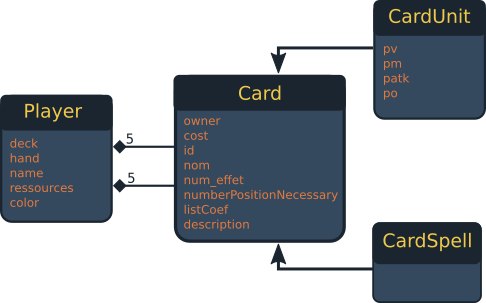
\includegraphics[scale=0.4]{Assets/umlBlocCarte.png}
            \caption{Zoom sur le bloc joueur}
            \label{fig7}
          \end{center}
        \end{figure}
             
          \subsection{Les joueurs}
            \begin{center}
            \textit{Classe : Player}
            \end{center}
            Les joueurs ont une <<main>> qui contient cinq cartes (attribut \textit{hand}), et un <<deck>> qui en contient cinq également (attribut \textit{deck}). Les joueurs possèdent également un nom,  une couleur (en chaine de caractères) et un nombre de ressources. C'est de cette classe que vont être jouées les cartes.
            
          \subsection{Jouer une carte}
            \begin{center}
            \textit{Classe : Player, Card - Fonction : doEffect() , playCard(),  spawn()}
            \end{center}
            La notion de jouer une carte va faire appelle à plusieurs engrenages du système.Tout d'abord la fonction \textit{playCard()} va récupérer une liste de coordonées construite par le controlleur en fonction de l'attribut \textit{nomberPositionNecessary} de la carte. Tout d'abord le programme va regarder si la carte peut-être jouée, c'est-à-dire si le joueur à le nombre de ressources nécessaire pour jouer la carte. Ensuite, l'algorithme va déterminer si la carte est une carte unité ou une carte sort. Si la carte est une unité, cette carte va créer l'unité en récupérant et enlevant la première position de la liste de position. Puis le traitement ce rejoint entre les deux types de carte en appelant la fonction \textit{doEffect()}.
            
          \subsection{Jouer un effet}
            \begin{center}
            \textit{Classe : Card - Fonction : doEffect()}
            \end{center}
            Jouer un effet est la partie qui lie le plus la base de données au jeu, et par conséquence, demande une grande rigueur dans l'insertion des effets et des cartes dans celle-ci. En effet, lors de l'appel à la méthode \textit{doEffect()}, celle-ci va regarder via l'attribut \textit{num\_effet} le numéros de l'effet, qui correspond à l'identifiant de celui-ci dans la base de données. En fonction de ce chiffre, la méthode va faire le traitement adapté à cette identifiant.

         \begin{figure}[th]
          \begin{center}
            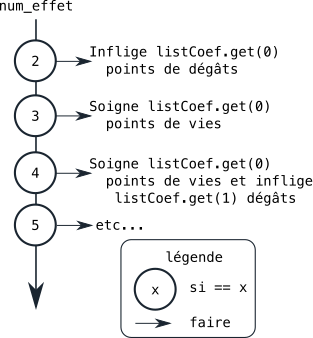
\includegraphics[scale=0.5]{Assets/decisionEffet.png}
            \caption{Schémas du traitement de la fonction \textit{doEffect()}}
            \label{decisionEffet}
          \end{center}
        \end{figure}
      
          \subsection{Mélanger les cartes}
            \begin{center}
            \textit{Classe : Player - Fonction : shuffle()}
            \end{center}
              La méthode \textit{shuffle()} va remettre toute les cartes dans le <<deck>> avant de les mélanger et de reprendre cinq cartes dans la <<main>>.
            
    \section{Le jeu}
     Nous allons maintenant parler de la classe \textit{Game}.
      
     \begin{figure}[th]
        \begin{center}
          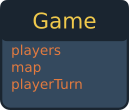
\includegraphics[scale=0.4]{Assets/UMLGame.png}
          \caption{Zoom sur la classe \textit{Game}}
          \label{figUMLGame}
        \end{center}
      \end{figure}
      
      \subsection{Savoir qui joue}
        \begin{center}
        \textit{Classe : Game - Fonction : getPlayerTurn()}
        \end{center}
        La classe \textit{Game} contient une liste de joueur ainsi qu'une variable appelée \textit{playerTurn}. Cette variable est utilisée comme un curseur qui indique quel élément de la liste doit jouer.

      \subsection{Récupération des cartes}
        \begin{center}
        \textit{Classe : Game - Fonction : setDeckPlayerByName()}
        \end{center}
        C'est le serveur qui est chargé de la récupération des cartes depuis la base de données. Il va ensuite les envoyer au jeu grâce à la méthode \textit{setDeckPlayerByName()}. Cette méthode prend le nom d'un joueur ainsi qu'un tableau de cartes en paramètre, et va donc ajouter celles-ci au joueur du modèle ayant ce nom. Si aucun joueur ne correspond, la fonction nous informe via un booléen de l'échec de la méthode.
        
        \subsection{Initialisation de la carte}
        \begin{center}
        \textit{Classe : Game - Fonction : initMap()}
        \end{center}
        La création de la carte ne dépend que d'un seul élément, le nombre de joueur. Selon celui-ci, la carte sera créés suivant un modèle codé dans le programme.
        
        \subsection{La gestion de la fin du tour}
        \begin{center}
        \textit{Classe : Game - Fonction : endTurn()}
        \end{center}
        La fonction \textit{endTurn()} est appelée à chaque fin de tour de façon à débloquer les unités du joueur (booléen \textit{sleep}), à remettre leurs points de mouvements à leurs maximums et de changer de joueur en incrémentant la variable \textit{playerTurn}. 
        
      \section{Les exceptions}
        Nous allons ici détailler les différentes exceptions propre au modèle.
        \begin{description}
          \item[EffectException : ]Déclenché lorsqu’un effet n’est pas utilisé dans de bonne condition, (exemple : les coordonnées sélectionnées ne contiennent pas d’unités).
          \item[MoveException : ]Déclenché lorsqu'une unité essaie de ce déplacer sur une case déjà occupé, ou qu'il ne peut pas atteindre.
          \item[PlayCardException : ]Déclenché si un joueur tente de jouer une carte qui coûte plus que le nombre de ressources dont il dispose.
          \item[RangeException : ]Déclenché par une unité qui tente d'attaquer une autre, qui n'est pas à sa portée.
          \item[SpawnExcpetion :]Déclenché par un joueur qui tente de poser une unité sur une case qui est déjà occupée ou qui n'appartient pas à celui-ci.
        \end{description}
        
        
\end{document}  
